\documentclass[11pt]{article}
% Useful math stuff in amsmath
\usepackage{amsmath}
% Graphicx for including pictures in various formats
\usepackage{graphicx}
%
\usepackage{fullpage}
% Tweak the headings
\pagestyle{myheadings}
\renewcommand{\thepage}{Page \arabic{page}}
\newcommand{\pagetop}{Team \# 46364}
\setlength{\headsep}{0.4in}
\markboth{\pagetop}{\pagetop}
%
% \T and \B are 'fudge factors' for the tabular environment.
%
\newcommand\T{\rule{0pt}{2.6ex}}
\newcommand\B{\rule[-1.2ex]{0pt}{0pt}}
%
% The main document begins here...
%
\begin{document}

\centerline{\textbf{\Large Title of the Report}}

\section{Introduction}

Here are examples of citing references. A classic reference on the
perturbation theory of linear operators is the text by Kato \cite{KATO}.
A discussion of the Runge-Kutta method can be found in most undergraduate
texts on numerical analysis \cite{BF,MF}.

Section \ref{sec:BG} describes some background material.
The amazing results of our analysis are given in Section \ref{sec:RESULTS}.

\section{Background}
\label{sec:BG}

Here is an example of a numbered equation.
\begin{equation}
\frac{dy}{dx} = x^2y
\label{DE}
\end{equation}
Equation~\eqref{DE} is a differential equation.
Here is an equation that is not numbered.
\[
   m\ddot{x} + \gamma \dot{x} + k x = 0.
\]
More complicated mathematical formulas are possible.
For example,
\[
\begin{pmatrix}
    1 & 2 & 3 \\
    0 & 4 & 5 \\
    0 & 0 & 6
\end{pmatrix}
\begin{pmatrix}
    x \\
    y \\
    z
\end{pmatrix}
  = \begin{pmatrix}
        \pi \\
        -\pi^2 \\
        \frac{1}{2}
     \end{pmatrix}
\]
This sentence will have a footnote.\footnote{This is the footnote!}


Here is an example of how to include a postscript file as a figure.
\begin{figure}[p]
\centerline{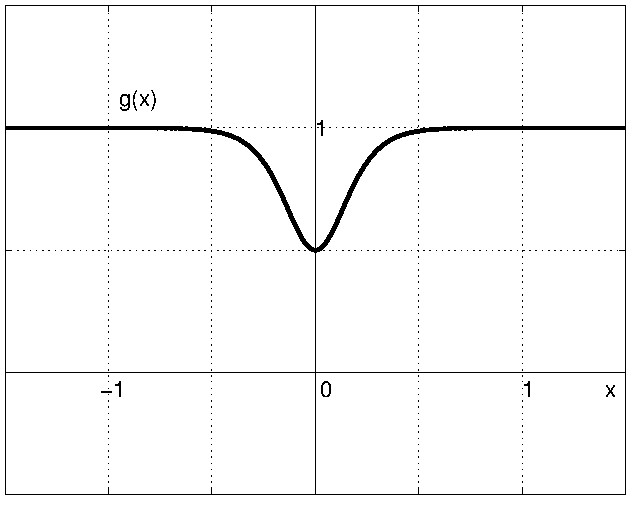
\includegraphics[width=3.5in]{myfile.jpg}}
\caption{This is an example of a figure that contains a postscript file.}
\label{FIG}
\end{figure}
You can refer to Figure \ref{FIG} using the same Latex command
that you use to refer to sections.
When you look at the Latex file, you will see that I used the
[p] option with the figure environment.  This tells Latex to
put the figure on a separate page.
You can experiment with other options (such as [h] for ``here''
and [b] for ``bottom of the current page'').

There are many more useful things that you can do in Latex.  For example,
here is a list of stuff:
\begin{itemize}
\item This is the first entry.
\item This is the second.
\item And so on...
\end{itemize}
Here is a numbered list:
\begin{enumerate}
\item This is the first entry.
\item This is the second.
\end{enumerate}

Here is an example of the \textbf{tabular} environment:

\centerline{%
\begin{tabular}{|r|r|r|}
\hline
$n$ & $n^2$ & $n!$ \T \\
\hline
1 &  1 & 1\\
2 &  4 & 2\\
3 &  9 & 6\\
4 & 16 & 24\\
5 & 25 & 120\\
6 & 36 & 720\\
7 & 49 & 5040\\
8 & 64 & 40320\\
\hline
\end{tabular}
} % end centerline
You might want to treat a table like this the same way that
a figure is treated.  For example, I have put the same data
into Table~\ref{table:DATA}.
\begin{table}
\centerline{%
\begin{tabular}{|r|r|r|}
\hline
$n$ & $n^2$ & $n!$ \T \\
\hline
1 &  1 & 1\\
2 &  4 & 2\\
3 &  9 & 6\\
4 & 16 & 24\\
5 & 25 & 120\\
6 & 36 & 720\\
7 & 49 & 5040\\
8 & 64 & 40320\\
\hline
\end{tabular}
} % end centerline
\caption{The values of $n!$ and $n^2$ for $n$ from $1$ to $8$.}
\label{table:DATA}
\end{table}
Notice how it was removed from the flow of the text and put
at the top of the page.




\section{Results}
\label{sec:RESULTS}

Ipsit sic nada quorum deluge France speaker only now for the end
it was Massachusetts.
Ipsit sic nada quorum deluge France speaker only now for the end
it was Massachusetts.
Ipsit sic nada quorum deluge France speaker only now for the end
it was Massachusetts.

Ipsit sic nada quorum deluge France speaker only now for the end
it was Massachusetts.
Ipsit sic nada quorum deluge France speaker only now for the end
it was Massachusetts.
Ipsit sic nada quorum deluge France speaker only now for the end
it was Massachusetts.

%
% Put the references here...
%
\begin{thebibliography}{99}
\bibitem{KATO} T.~Kato, \emph{Perturbation Theory for Linear Operators}, Springer-Verlag,
                  Berlin, 1980.
\bibitem{BF} R.~L.~Burden, J.~D.~Faires, \emph{Numerical Analysis (fifth edition)},
                  PWS Publishing Company, Boston, 1993.
\bibitem{MF} J.~H.~Mathews, K.~D.~Fink, \emph{Numerical Methods Using MATLAB (third edition)},
                  Prentice-Hall, New Jersey, 1999.
\end{thebibliography}

\end{document}
